

\input{../Latex_Templates/Preamble_Report}

%%%%% TITLE PAGE

%\subject{, VT23}
\title{ Report for the Course Modelling in Computational Science, HT23 \\[1ex]
	  \large Project 1: The Potts model}
%\subtitle{}
\author{Theo Koppenhöfer}
\date{Lund \\[1ex] \today}

\addbibresource{bibliography.bib}

\usepackage{pythonhighlight}
\usepackage{pgfplots}
\graphicspath{{../Figures/}}

\pgfplotsset{
	compat=newest,
    every axis/.append style={
        axis y line=left,
        axis x line=bottom,
        scale only axis,
%    	max space between ticks=25pt,
        width=\textwidth,
        scaled ticks=true,
        axis line style={thick,-,>=latex, shorten >=-.4cm},
    		x tick label style={
		    /pgf/number format/precision=3
		}
    },
    every axis plot/.append style={thick},
    tick style={black, thick}
}

%%%%% The content starts here %%%%%%%%%%%%%


\begin{document}

\maketitle

\section{Introduction}

The following report is part of the first project of the Modelling in Computational Science course at Lund University, HT2023.
In the first project we implemented a Monte-Carlo simulation of the $q$-state Potts model.
The report and the Python implementation can be found online under \cite{Repository}

\section{The Potts model}

The following is a brief introduction to the potts model from statistical mechanics.
A state of the $q$-state Potts model of a $L\times L$ flat grid is given by a mapping
\begin{align*}
	s\colon \brk[c]{1,\dots,L}\times\brk[c]{1,\dots,L}\to\brk[c]{1,\dots,L}\,.
\end{align*}
One assigns this state an energy via
\begin{align*}
	E = -J\sum_{\substack{i, j\text{ neighbouring}\\ \text{grid points}}}\delta\brk*{s_i,s_j}
\end{align*}
where $\delta$ denotes the Kronecker-delta and $J=1$ is the coupling strength. As given in the problem setting we assume periodic boundary conditions on the grid.

\section{The algorithms}

To model the statistical behaviour of the model we use Monte-Carlo simulations. 
The first method we implemented was the Metropolis algorithm.
The steps for the Metropolis algorithm are given in figure \ref{alg:Metropolis}. A single iteration of this algorithm is performed by the function \pyth{MC_step_fast} in the implementation. In the implementation we used the pseudo-random number generators from \pyth{numpy.random} for the proposed spins, spin states and for determining if the choice should be accepted.

\begin{figure}
\centering
\begin{algorithm}[H]
\caption{Metropolis}
\label{alg:Metropolis}
\SetKwInOut{Input}{Input}

\Input{Initial data $s$, $L$, $T$, $q$}
\BlankLine
\For{$k=0,1,\dots$}{
	Pick a point on the grid.
	
	Propose a new random spin value for this point.
	
	Calculate the change of energy $\Delta E$ that this spin flip would cause.
	
	Accept this spin flip with probability $\min\brk[c]*{1,\exp(-\Delta E/T)}$.
}
\end{algorithm}
\end{figure}

Analogously to the Metropolis algorithm the steps of the heat-bath algorithm are given in figure \ref{alg:heat-bath}. it differs from the Metropolis algorithm only after a point on the grid was randomly chosen. In the implementation a single iteration is performed by the function \pyth{Gibbs_step}. In the implementation for this algorithm we also used the \pyth{numpy.random} functions.

\begin{figure}
\centering
\begin{algorithm}[H]
\caption{Heat-bath}
\label{alg:heat-bath}
\SetKwInOut{Input}{Input}

\Input{Initial data $s$, $L$, $T$, $q$}
\BlankLine
\For{$k=0,1,\dots$}{
	Pick a point on the grid.
	
	Pick a spin value for this point with a probability given by the distribution
	\begin{align*}
		p(s_i) = C \exp\brk*{\frac{1}{T}\sum_{j\text{ neighbours }i}\delta\brk*{s_i,s_j}}\,.
	\end{align*}
	Here $C$ is a normalisation constant.
}
\end{algorithm}
\end{figure}

\section{Some implementation details}

\subsubsection{Determining when the Energy has plateaued}

In order for the simulation to start sampling we needed a criteria to determine the time $t_0$ when the system reaches an equilibrium state.
 To determine $t_0$ we calculate in every step $i$ moving averages $\text{ma}_1$ and $\text{ma}_2$ over $n$ energies. The construction is shown in figure \ref{fi:movingAverages}. If we start in the hot state then the energy will tend to decrease until we reach an equilibrium. Hence we can use the condition
\begin{align}
	\text{ma}_2 \leq \text{ma}_1 \label{eq:equilCondition}
\end{align}
to determine $t_0$. If on the other hand we start in cold state the energy will in general increase and we have to reverse the inequality in equation \eqref{eq:equilCondition}. After reaching an equilibrium the simulation runs for a further \pyth{M_sampling} steps. It is over these samples we take the mean and the standard deviation.

\begin{figure}
\centering
\input{../Figures/explanationMovingAverages.pdf_tex}
\caption{A visualisation of the moving averages.}
\label{fi:movingAverages}
\end{figure}

\subsubsection{Improving performance}

While simulating we run into performance issues due to the fact that Python is in general rather slow even with heavy use of \pyth{numpy}. We resolved this issue with the help of \pyth{numba} which precompiled functions and thus increased performance substantially. The downside is that the code becomes quite unaestetic because \pyth{numba} does not support all \pyth{python} and \pyth{numpy} features. In hindsight it would probably been better to have written the iteration in a language other than python.
In the experiments we also preferred to use the Metropolis algorithm because our implementation of this algorithm ran faster than the heat-bath algorithm.

\section{The experiments}

\subsection{A brief sanity check}

In order to check that our code was indeed doing what it was supposed to we designed some sanity checks. 
The energy during the simulation is updated with the calculated value for $\Delta E$.
Hence we checked with the function \pyth{test_energies} if the energy of the end state of the simulation is the same as the energy calculated during the simulation.

We also ran the simulation



\subsection{State plots}

In figures \ref{fi:Low_temp_state} to \ref{fi:High_temp_state} we can see that as the temperature increases the state of the system becomes more chaotic. For low temperatures there are larger patches of the same state which corresponds to a lower energy configuration. In the implementation one can see an animated version of the evolution of the system state.

\begin{figure}
\begin{minipage}{0.25\textwidth}
\centering
\graphicspath{{../../Plots/}}
% This file was created with tikzplotlib v0.10.1.
\begin{tikzpicture}

\definecolor{darkgray176}{RGB}{176,176,176}

\begin{axis}[
tick align=outside,
tick pos=left,
x grid style={darkgray176},
xmin=-0.5, xmax=19.5,
xtick style={color=black},
y dir=reverse,
y grid style={darkgray176},
ymin=-0.5, ymax=19.5,
ytick style={color=black}
]
\addplot graphics [includegraphics cmd=\pgfimage,xmin=-0.5, xmax=19.5, ymin=19.5, ymax=-0.5] {High_temp_state_10000-001.png};
\end{axis}

\end{tikzpicture}

\caption{State for temperature $T=0.1$.}
\label{fi:High_temp_state}
\end{minipage}
\hfill
\begin{minipage}{0.25\textwidth}
\centering
\graphicspath{{../../Plots/}}
\input{../../Plots/Medium_temp_state_10000.pgf}
\caption{State for temperature $T=1$.}
\label{fi:Medium_temp_state}
\end{minipage}
\hfill
\begin{minipage}{0.25\textwidth}
\centering
\graphicspath{{../../Plots/}}
% This file was created with tikzplotlib v0.10.1.
\begin{tikzpicture}

\definecolor{lightgray}{RGB}{211,211,211}

\begin{axis}[
tick align=outside,
tick pos=left,
x grid style={lightgray},
xmajorgrids,
xmin=-0.5, xmax=19.5,
xtick style={color=black},
y dir=reverse,
y grid style={lightgray},
ymajorgrids,
ymin=-0.5, ymax=19.5,
ytick style={color=black}
]
\addplot graphics [includegraphics cmd=\pgfimage,xmin=-0.5, xmax=19.5, ymin=19.5, ymax=-0.5] {../../Plots/Low_temp_state_10000-002.png};
\end{axis}

\end{tikzpicture}

\caption{State for temperature $T=100$.}
\label{fi:Low_temp_state}
\end{minipage}
\end{figure}



\subsection{Distribution of energies in equilibrium}

In the following numerical experiment we set the grid size to $L=300$, the spin states to $q=10$ and the temperature to $T=10^2$. We then run the simulation until the system reached equilibrium. After that we varied the number of steps $M$ of the simulation and plotted the distribution of energies. The results can be seen in figures \ref{pl:Maxwell_distribution_0} to \ref{pl:Maxwell_distribution_3}. One sees that as $M$ increases the distribution approaches the Maxwell-Boltzmann distribution.

\begin{figure}
\begin{minipage}[b]{0.4\textwidth}
\centering
\input{../../Plots/Energies_maxwell_distribution_MC_step_fast_T1_0.pgf}
\vspace*{-0.5cm}
\caption{For $M=10^5$}
\label{pl:Maxwell_distribution_0}
\end{minipage}
\hfill
\begin{minipage}[b]{0.4\textwidth}
\centering
\input{../../Plots/Energies_maxwell_distribution_MC_step_fast_T1_1.pgf}
\vspace*{-0.5cm}
\caption{For $M=10^6$}
\label{pl:Maxwell_distribution_1}
\end{minipage}
\begin{minipage}[b]{0.4\textwidth}
\vspace*{1cm}
\centering
\input{../../Plots/Energies_maxwell_distribution_MC_step_fast_T1_2.pgf}
\vspace*{-0.5cm}
\caption{For $M=4\cdot10^6$}
\label{pl:Maxwell_distribution_2}
\end{minipage}
\hfill
\begin{minipage}[b]{0.4\textwidth}
\centering
\input{../../Plots/Energies_maxwell_distribution_MC_step_fast_T1_3.pgf}
\vspace*{-0.5cm}
\caption{For $M=10^7$}
\label{pl:Maxwell_distribution_3}
\end{minipage}
\end{figure}

\subsection*{Energies in dependence of the temperature}

In this experiment we plotted the energies in dependence of the temperature for a system with parameters $q=2$ and $q=10$. Our aim was to see the critical temperature $T_c=1/(\ln(1+\sqrt{q})$. For this we wanted to simulate a system of maximal size. Since a sampling size beyond $10^7$ seemed unreasonable and the temperature would be in the region of $T\approx1$ the previous experiment suggested a maximal system size of $L=50$. For larger systems the distribution plot shown in figure \ref{pl:Maxwell_distribution_3} would become degenerate.
So we run the experiment with a sampling size of \pyth{M_sampling=10E7} and chose the parameter $n$ for the moving averages to be $10^6$. The results of the experiment are shown in plot. The error bars in the plot are the standard deviation of the energies.

\begin{figure}
\centering
\begin{minipage}{0.7\textwidth}
\centering
\graphicspath{{../../Plots/}}
% This file was created with tikzplotlib v0.10.1.
\begin{tikzpicture}

\definecolor{darkgray176}{RGB}{176,176,176}
\definecolor{darkorange25512714}{RGB}{255,127,14}
\definecolor{lightgray204}{RGB}{204,204,204}
\definecolor{steelblue31119180}{RGB}{31,119,180}

\begin{axis}[
legend cell align={left},
legend style={
  fill opacity=0.8,
  draw opacity=1,
  text opacity=1,
  at={(0.03,0.97)},
  anchor=north west,
  draw=lightgray204
},
tick align=outside,
tick pos=left,
x grid style={darkgray176},
xlabel={Temperature \(\displaystyle T\)},
xmin=-0.0895, xmax=2.0995,
xtick style={color=black},
y grid style={darkgray176},
ylabel={Energy \(\displaystyle E\) per spin},
ymin=-2.09902319979481, ymax=-0.214846733941415,
ytick style={color=black}
]
\path [draw=steelblue31119180, semithick]
(axis cs:0.01,-2.00940159517146)
--(axis cs:0.01,-1.98053700898854);

\path [draw=steelblue31119180, semithick]
(axis cs:0.0786206896551724,-2.01206615830345)
--(axis cs:0.0786206896551724,-1.97255869993655);

\path [draw=steelblue31119180, semithick]
(axis cs:0.147241379310345,-2.0087859287851)
--(axis cs:0.147241379310345,-1.9826953875349);

\path [draw=steelblue31119180, semithick]
(axis cs:0.215862068965517,-1.96269947602565)
--(axis cs:0.215862068965517,-1.95439161885435);

\path [draw=steelblue31119180, semithick]
(axis cs:0.28448275862069,-2.0133788149833)
--(axis cs:0.28448275862069,-1.9672730480567);

\path [draw=steelblue31119180, semithick]
(axis cs:0.353103448275862,-2.01102362026044)
--(axis cs:0.353103448275862,-1.97810517397956);

\path [draw=steelblue31119180, semithick]
(axis cs:0.421724137931034,-1.95642239362181)
--(axis cs:0.421724137931034,-1.94641077373819);

\path [draw=steelblue31119180, semithick]
(axis cs:0.490344827586207,-1.95509234848907)
--(axis cs:0.490344827586207,-1.93856055055093);

\path [draw=steelblue31119180, semithick]
(axis cs:0.558965517241379,-1.95244412952991)
--(axis cs:0.558965517241379,-1.92684634183009);

\path [draw=steelblue31119180, semithick]
(axis cs:0.627586206896552,-2.00787321174421)
--(axis cs:0.627586206896552,-1.95082735865579);

\path [draw=steelblue31119180, semithick]
(axis cs:0.696206896551724,-1.99607514880384)
--(axis cs:0.696206896551724,-1.93737911519616);

\path [draw=steelblue31119180, semithick]
(axis cs:0.764827586206897,-1.99208733869643)
--(axis cs:0.764827586206897,-1.92695562370357);

\path [draw=steelblue31119180, semithick]
(axis cs:0.833448275862069,-1.96930870654393)
--(axis cs:0.833448275862069,-1.88345143489607);

\path [draw=steelblue31119180, semithick]
(axis cs:0.902068965517241,-1.94399639218978)
--(axis cs:0.902068965517241,-1.87372839965022);

\path [draw=steelblue31119180, semithick]
(axis cs:0.970689655172414,-1.84665120146144)
--(axis cs:0.970689655172414,-1.79402292445856);

\path [draw=steelblue31119180, semithick]
(axis cs:1.03931034482759,-1.8593794685843)
--(axis cs:1.03931034482759,-1.7786811907757);

\path [draw=steelblue31119180, semithick]
(axis cs:1.10793103448276,-1.78068222462622)
--(axis cs:1.10793103448276,-1.71493306129378);

\path [draw=steelblue31119180, semithick]
(axis cs:1.17655172413793,-1.67309706784008)
--(axis cs:1.17655172413793,-1.60902290223992);

\path [draw=steelblue31119180, semithick]
(axis cs:1.2451724137931,-1.58160008264805)
--(axis cs:1.2451724137931,-1.53389484551195);

\path [draw=steelblue31119180, semithick]
(axis cs:1.31379310344828,-1.52874150433815)
--(axis cs:1.31379310344828,-1.48430522174185);

\path [draw=steelblue31119180, semithick]
(axis cs:1.38241379310345,-1.48479427459037)
--(axis cs:1.38241379310345,-1.44423605708963);

\path [draw=steelblue31119180, semithick]
(axis cs:1.45103448275862,-1.45024455588998)
--(axis cs:1.45103448275862,-1.41011223291002);

\path [draw=steelblue31119180, semithick]
(axis cs:1.51965517241379,-1.42005529211439)
--(axis cs:1.51965517241379,-1.38107419220561);

\path [draw=steelblue31119180, semithick]
(axis cs:1.58827586206897,-1.39604890931988)
--(axis cs:1.58827586206897,-1.35893581228012);

\path [draw=steelblue31119180, semithick]
(axis cs:1.65689655172414,-1.37295550071337)
--(axis cs:1.65689655172414,-1.33750580312663);

\path [draw=steelblue31119180, semithick]
(axis cs:1.72551724137931,-1.35322149902781)
--(axis cs:1.72551724137931,-1.31879512657219);

\path [draw=steelblue31119180, semithick]
(axis cs:1.79413793103448,-1.33579052985162)
--(axis cs:1.79413793103448,-1.30200083590838);

\path [draw=steelblue31119180, semithick]
(axis cs:1.86275862068966,-1.31987105835943)
--(axis cs:1.86275862068966,-1.28592159972057);

\path [draw=steelblue31119180, semithick]
(axis cs:1.93137931034483,-1.30777567147544)
--(axis cs:1.93137931034483,-1.27345731028456);

\path [draw=steelblue31119180, semithick]
(axis cs:2,-1.29532325951322)
--(axis cs:2,-1.26224049360678);

\path [draw=darkorange25512714, semithick]
(axis cs:0.01,-1.78606053584287)
--(axis cs:0.01,-1.76000525191713);

\path [draw=darkorange25512714, semithick]
(axis cs:0.0786206896551724,-1.80311228677963)
--(axis cs:0.0786206896551724,-1.74973973666037);

\path [draw=darkorange25512714, semithick]
(axis cs:0.147241379310345,-1.81918330626443)
--(axis cs:0.147241379310345,-1.76175206885557);

\path [draw=darkorange25512714, semithick]
(axis cs:0.215862068965517,-1.85117515060571)
--(axis cs:0.215862068965517,-1.76970440739429);

\path [draw=darkorange25512714, semithick]
(axis cs:0.28448275862069,-1.88627252085735)
--(axis cs:0.28448275862069,-1.80798781034265);

\path [draw=darkorange25512714, semithick]
(axis cs:0.353103448275862,-1.91107799238211)
--(axis cs:0.353103448275862,-1.78332124553789);

\path [draw=darkorange25512714, semithick]
(axis cs:0.421724137931034,-1.90177833454075)
--(axis cs:0.421724137931034,-1.73889506369925);

\path [draw=darkorange25512714, semithick]
(axis cs:0.490344827586207,-1.88452799961117)
--(axis cs:0.490344827586207,-1.72979172046883);

\path [draw=darkorange25512714, semithick]
(axis cs:0.558965517241379,-1.8648574769578)
--(axis cs:0.558965517241379,-1.6610116048822);

\path [draw=darkorange25512714, semithick]
(axis cs:0.627586206896552,-1.76418205792112)
--(axis cs:0.627586206896552,-1.45235329847888);

\path [draw=darkorange25512714, semithick]
(axis cs:0.696206896551724,-1.12021842301625)
--(axis cs:0.696206896551724,-0.972847966103754);

\path [draw=darkorange25512714, semithick]
(axis cs:0.764827586206897,-0.73236574961624)
--(axis cs:0.764827586206897,-0.69167163006376);

\path [draw=darkorange25512714, semithick]
(axis cs:0.833448275862069,-0.62661217094774)
--(axis cs:0.833448275862069,-0.59270813457226);

\path [draw=darkorange25512714, semithick]
(axis cs:0.902068965517241,-0.566062025690209)
--(axis cs:0.902068965517241,-0.535288838149791);

\path [draw=darkorange25512714, semithick]
(axis cs:0.970689655172414,-0.519107970834819)
--(axis cs:0.970689655172414,-0.491374024765181);

\path [draw=darkorange25512714, semithick]
(axis cs:1.03931034482759,-0.485503696018345)
--(axis cs:1.03931034482759,-0.458181817101655);

\path [draw=darkorange25512714, semithick]
(axis cs:1.10793103448276,-0.459916510894878)
--(axis cs:1.10793103448276,-0.433728776705122);

\path [draw=darkorange25512714, semithick]
(axis cs:1.17655172413793,-0.437479165067947)
--(axis cs:1.17655172413793,-0.412369172372053);

\path [draw=darkorange25512714, semithick]
(axis cs:1.2451724137931,-0.418514483901034)
--(axis cs:1.2451724137931,-0.394547800658966);

\path [draw=darkorange25512714, semithick]
(axis cs:1.31379310344828,-0.403170304467868)
--(axis cs:1.31379310344828,-0.379694590972132);

\path [draw=darkorange25512714, semithick]
(axis cs:1.38241379310345,-0.390499655259397)
--(axis cs:1.38241379310345,-0.367244183540603);

\path [draw=darkorange25512714, semithick]
(axis cs:1.45103448275862,-0.378600006014082)
--(axis cs:1.45103448275862,-0.355714834385918);

\path [draw=darkorange25512714, semithick]
(axis cs:1.51965517241379,-0.36839129602659)
--(axis cs:1.51965517241379,-0.34604471717341);

\path [draw=darkorange25512714, semithick]
(axis cs:1.58827586206897,-0.35927669292776)
--(axis cs:1.58827586206897,-0.33738325579224);

\path [draw=darkorange25512714, semithick]
(axis cs:1.65689655172414,-0.351371610282304)
--(axis cs:1.65689655172414,-0.329601259957696);

\path [draw=darkorange25512714, semithick]
(axis cs:1.72551724137931,-0.343473264452733)
--(axis cs:1.72551724137931,-0.322143550907267);

\path [draw=darkorange25512714, semithick]
(axis cs:1.79413793103448,-0.337556999047295)
--(axis cs:1.79413793103448,-0.316194152792705);

\path [draw=darkorange25512714, semithick]
(axis cs:1.86275862068966,-0.331522904947437)
--(axis cs:1.86275862068966,-0.310428247292563);

\path [draw=darkorange25512714, semithick]
(axis cs:1.93137931034483,-0.326816603104549)
--(axis cs:1.93137931034483,-0.305982922655451);

\path [draw=darkorange25512714, semithick]
(axis cs:2,-0.321308818927067)
--(axis cs:2,-0.300491118752933);

\addplot [semithick, steelblue31119180]
table {%
0.01 -1.99496930208
0.0786206896551724 -1.99231242912
0.147241379310345 -1.99574065816
0.215862068965517 -1.95854554744
0.28448275862069 -1.99032593152
0.353103448275862 -1.99456439712
0.421724137931034 -1.95141658368
0.490344827586207 -1.94682644952
0.558965517241379 -1.93964523568
0.627586206896552 -1.9793502852
0.696206896551724 -1.966727132
0.764827586206897 -1.9595214812
0.833448275862069 -1.92638007072
0.902068965517241 -1.90886239592
0.970689655172414 -1.82033706296
1.03931034482759 -1.81903032968
1.10793103448276 -1.74780764296
1.17655172413793 -1.64105998504
1.2451724137931 -1.55774746408
1.31379310344828 -1.50652336304
1.38241379310345 -1.46451516584
1.45103448275862 -1.4301783944
1.51965517241379 -1.40056474216
1.58827586206897 -1.3774923608
1.65689655172414 -1.35523065192
1.72551724137931 -1.3360083128
1.79413793103448 -1.31889568288
1.86275862068966 -1.30289632904
1.93137931034483 -1.29061649088
2 -1.27878187656
};
\addlegendentry{10}
\addplot [semithick, darkorange25512714]
table {%
0.01 -1.77303289388
0.0786206896551724 -1.77642601172
0.147241379310345 -1.79046768756
0.215862068965517 -1.810439779
0.28448275862069 -1.8471301656
0.353103448275862 -1.84719961896
0.421724137931034 -1.82033669912
0.490344827586207 -1.80715986004
0.558965517241379 -1.76293454092
0.627586206896552 -1.6082676782
0.696206896551724 -1.04653319456
0.764827586206897 -0.71201868984
0.833448275862069 -0.60966015276
0.902068965517241 -0.55067543192
0.970689655172414 -0.5052409978
1.03931034482759 -0.47184275656
1.10793103448276 -0.4468226438
1.17655172413793 -0.42492416872
1.2451724137931 -0.40653114228
1.31379310344828 -0.39143244772
1.38241379310345 -0.3788719194
1.45103448275862 -0.3671574202
1.51965517241379 -0.3572180066
1.58827586206897 -0.34832997436
1.65689655172414 -0.34048643512
1.72551724137931 -0.33280840768
1.79413793103448 -0.32687557592
1.86275862068966 -0.32097557612
1.93137931034483 -0.31639976288
2 -0.31089996884
};
\addlegendentry{10}
\end{axis}

\end{tikzpicture}

\caption{}
\label{fi:energies_T_q_L50}
\end{minipage}
\end{figure}

We can see from figure \ref{fi:t0_T_q_L50} that it takes the simulation in most cases roughly $0.25\cdot 10^7$ steps to reach an equilibrium. For cold temperatures with $q=10$ this takes however far longer since the system starts in the 'hot' state.

\begin{figure}
\centering
\begin{minipage}{0.7\textwidth}
\centering
\graphicspath{{../../Plots/}}
% This file was created with tikzplotlib v0.10.1.
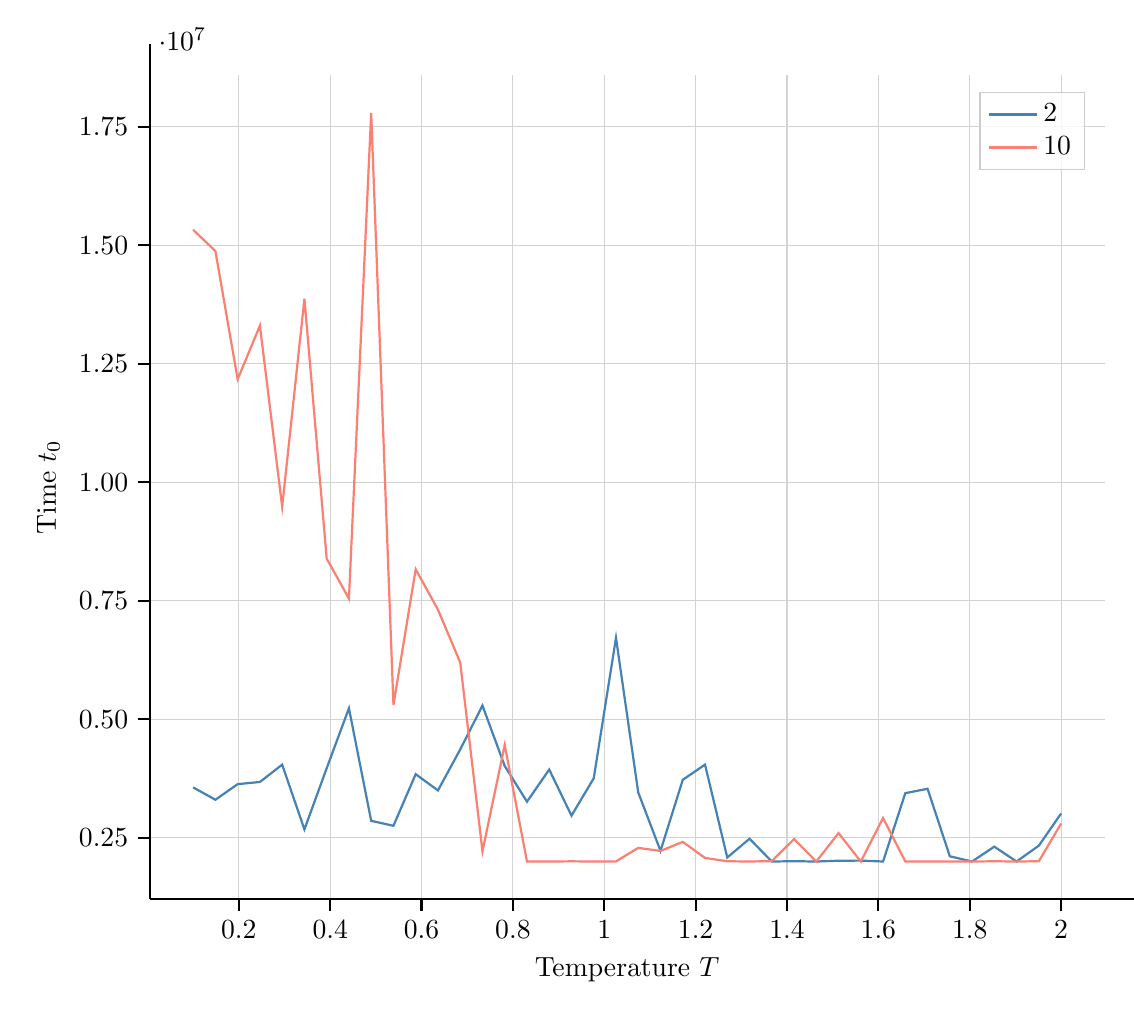
\begin{tikzpicture}

\definecolor{lightgray}{RGB}{211,211,211}
\definecolor{lightgray204}{RGB}{204,204,204}
\definecolor{salmon}{RGB}{250,128,114}
\definecolor{steelblue}{RGB}{70,130,180}

\begin{axis}[
legend cell align={left},
legend style={fill opacity=0.8, draw opacity=1, text opacity=1, draw=lightgray204},
tick align=outside,
tick pos=left,
x grid style={lightgray},
xlabel={Temperature \(\displaystyle T\)},
xmajorgrids,
xmin=0.005, xmax=2.095,
xtick style={color=black},
y grid style={lightgray},
ylabel={Time \(\displaystyle t_0\)},
ymajorgrids,
ymin=1210481, ymax=18579921,
ytick style={color=black},
ytick={0,2500000,5000000,7500000,10000000,12500000,15000000,17500000,20000000},
yticklabels={0.00,0.25,0.50,0.75,1.00,1.25,1.50,1.75,2.00}
]
\addplot [steelblue]
table {%
0.1 3563179
0.148717948717949 3302785
0.197435897435897 3632016
0.246153846153846 3677853
0.294871794871795 4043394
0.343589743589744 2677150
0.392307692307692 3966569
0.441025641025641 5231591
0.48974358974359 2858160
0.538461538461538 2753587
0.587179487179487 3842305
0.635897435897436 3499368
0.684615384615385 4363237
0.733333333333333 5289906
0.782051282051282 4015264
0.830769230769231 3261453
0.879487179487179 3939160
0.928205128205128 2967674
0.976923076923077 3755458
1.02564102564103 6717707
1.07435897435897 3454313
1.12307692307692 2224714
1.17179487179487 3723473
1.22051282051282 4043594
1.26923076923077 2084588
1.31794871794872 2480756
1.36666666666667 2000001
1.41538461538462 2006547
1.46410256410256 2000001
1.51282051282051 2016662
1.56153846153846 2019093
1.61025641025641 2000001
1.65897435897436 3442080
1.70769230769231 3534265
1.75641025641026 2109955
1.80512820512821 2000001
1.85384615384615 2313200
1.9025641025641 2000001
1.95128205128205 2335051
2 3012301
};
\addlegendentry{2}
\addplot [salmon]
table {%
0.1 15324519
0.148717948717949 14875805
0.197435897435897 12171568
0.246153846153846 13301926
0.294871794871795 9481749
0.343589743589744 13871093
0.392307692307692 8390135
0.441025641025641 7545768
0.48974358974359 17790401
0.538461538461538 5300741
0.587179487179487 8163350
0.635897435897436 7312571
0.684615384615385 6197677
0.733333333333333 2216463
0.782051282051282 4458079
0.830769230769231 2000001
0.879487179487179 2000001
0.928205128205128 2004020
0.976923076923077 2000001
1.02564102564103 2001599
1.07435897435897 2288168
1.12307692307692 2222709
1.17179487179487 2414126
1.22051282051282 2074911
1.26923076923077 2005394
1.31794871794872 2000001
1.36666666666667 2008848
1.41538461538462 2472908
1.46410256410256 2000001
1.51282051282051 2598966
1.56153846153846 2000001
1.61025641025641 2917558
1.65897435897436 2000001
1.70769230769231 2000001
1.75641025641026 2000001
1.80512820512821 2000001
1.85384615384615 2004943
1.9025641025641 2000001
1.95128205128205 2005701
2 2800493
};
\addlegendentry{10}
\end{axis}

\end{tikzpicture}

\caption{Time $t_0$ until the equilibrium is reached.}
\label{fi:t0_T_q_L50}
\end{minipage}
\end{figure}

In another series of experiments we would like to see how this plot depends on the system size $L$. The results can be seen in plots for system sizes $L=10$ and $L=30$.

\begin{figure}
\centering
\begin{minipage}{0.7\textwidth}
\centering
\graphicspath{{../../Plots/}}
\input{../../Plots/energies_T_q_L10.pgf}
\caption{$L=10$.}
\label{fi:energies_T_q_L50}
\end{minipage}
\end{figure}

\begin{figure}
\centering
\begin{minipage}{0.7\textwidth}
\centering
\graphicspath{{../../Plots/}}
\input{../../Plots/energies_T_q_L30.pgf}
\caption{$L=30$.}
\label{fi:energies_T_q_L50}
\end{minipage}
\end{figure}


\subsection{Plotting the energy distribution around the critical temperature}

In a final experiment we plotted the distribution of energies around the critical temperature for a grid size of $L=50$ and parameter $q=10$. The number of sampling steps was taken to be $M_sampling=10^8$. In figure \ref{fi:T0697} we see that the distribution of energies splits up at the temperature $T=0.697$. In figure \ref{fi:T0696} the distribution has shifted to the left for the slightly lower temperature $T=0.696$. 
Correspondingly for the slightly higher temperature $T=0.698$ we see in figure \ref{fi:T0698} that the distribution has shifted to the right.

\begin{figure}
\centering
\begin{minipage}{0.7\textwidth}
\centering
\graphicspath{{../../Plots/}}
\input{../../Plots/Energies_maxwell_distribution_MC_step_fast_T0.697_4.pgf}
\caption{Distribution of energies for the temperature $T=0.697$.}
\label{fi:T0697}
\end{minipage}
\end{figure}

\begin{figure}
\centering
\begin{minipage}[b]{0.45\textwidth}
\centering
\graphicspath{{../../Plots/}}
\input{../../Plots/Energies_maxwell_distribution_MC_step_fast_T0.696_4.pgf}
\caption{Distribution of energies for the temperature  $T=0.696$.}
\label{fi:T0696}
\end{minipage}
\hfill
\begin{minipage}[b]{0.45\textwidth}
\centering
\graphicspath{{../../Plots/}}
\input{../../Plots/Energies_maxwell_distribution_MC_step_fast_T0.698_4.pgf}
\caption{Distribution of energies for the temperature  $T=0.698$.}
\label{fi:T0698}
\end{minipage}
\end{figure}



\newpage
TODO:
\begin{itemize}
\item sanity test hot vs. cold start
\item energy evolution for maxwell-distribution test
\item phase transition test -> E-T plots and t0 plot
\item distribution based on energy
\item spell-check
\end{itemize}


\newpage
\section*{Bibliography}
%\nocite{*}
%Main source
%\printbibliography[heading=none, keyword={main}]
%\noindent Other sources
\printbibliography[heading=none, keyword={secondary}]

\end{document}
